\section{Preprocessing coastal data}
\label{sec:Preprocessing}
The SSH in the model is relative to
the reference geoid\footnote{the surface that a homogeneous static fluid would occupy
on an azimuthally symmetric Earth of the same size and rotation frequency}.
Dynamic topography emerges because of the
currents and density contrasts (Figures~\ref{fig:zos}~\&~\ref{fig:ssh_stats_america}A).

\begin{figure}
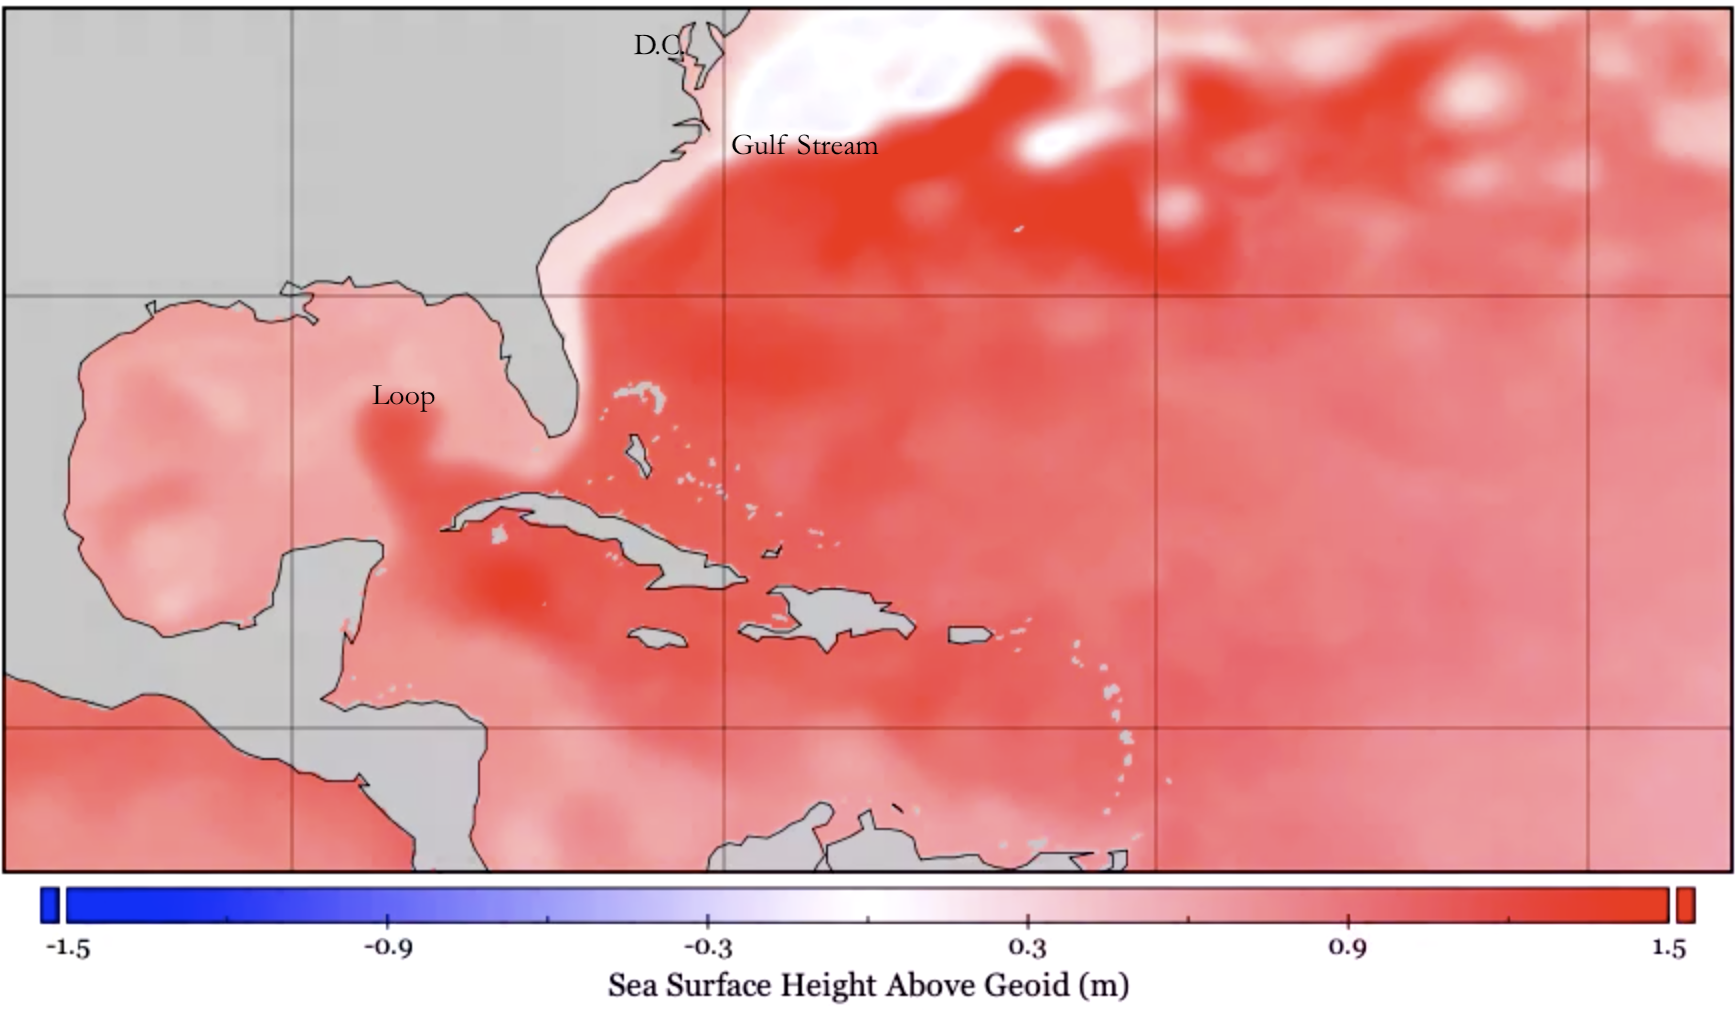
\includegraphics[width=\linewidth]{images/example-images/zos-image.png}
Sea Surface Height above Reference Geoid (\texttt{zos}, $\eta$, SSH)
\label{fig:zos}
\end{figure}




We define the third  moment around the mean,

\begin{equation}
\operatorname{Skew}[X]\equiv \mathbb{E}\left[\left(\frac{X-\mu}{\sigma}\right)^{3}\right]
=\frac{\mathbb{E}\left[(X-\mu)^{3}\right]}{\left(\mathbb{E}\left[(X-\mu)^{2}\right]\right)^{3 / 2}},
\end{equation}

and fourth as the excess above the Gaussian~\cite{taleb2019statistical},

\begin{equation}
\operatorname{Kurt}[X]=
\mathbb{E}\left[\left(\frac{X-\mu}{\sigma}\right)^{4}\right]-3
\equiv \frac{\mathbb{E}\left[(X-\mu)^{4}\right]}{\left(\mathbb{E}\left[(X-\mu)^{2}\right]\right)^{2}}-3.
\end{equation}




\begin{figure*}[htb!]
    \centering
    \includegraphics[width=0.6\linewidth]{../surge/plots/stats_points_plot.pdf}
       \hspace{0pt} \includegraphics[width=0.285\linewidth]{../surge/plots/stats_points_plot_1.pdf}
    \vspace{-7pt}
    \caption{A comparison between the distributions of sea surface height, $\eta$ (SSH/zos).
     above geoid for 2005 (red) and 2004 (blue),
     with the Pearson correlation coefficient, $r_p$, for each moment between the two years in A--D.
     Kurtosis in frame D is the excess above that expected for a normal distribution,
     which shows that areas like NO are highly non-normal (a statistical test
     shows that the probability of it being sampled from a Gaussian is $<10^{-304}$)~\cite{anscombe1983distribution}.
     An artefact in the data is that the mean of all of the points for the coastline
     seems to be uniformly shifted upwards between the two years (A~\&~E),
     where the difference is $0.06\pm0.01$m. }
   \label{fig:ssh_stats_america}
\end{figure*}



These are useful to summarise the SSH statistics
for \texttt{eUS} in Figure~\ref{fig:ssh_stats_america}.\footnote{
The individual points' SSH (Figure~\ref{fig:individual_zos} in §~\ref{sec:sum-var-stat}),
do not reveal any discontinuity in the data in \texttt{tyr},
 but Figures~\ref{fig:four-trans-panels}-\ref{fig:mm-hp-lp}
suggest that the displacement might be caused by \texttt{tyr} spin up from the
initial conditions.
}
On the right of panels \ref{fig:ssh_stats_america}A--D
is the Pearson regression coefficient, $r_p$,
between the two years for that moment, which shows that the mean and
std~dev of a point are c.~static between the years,
but the higher order moments of skew and kurtosis
(\ref{fig:ssh_stats_america}~C~\&~D) are more sensitive to the
random incidence of storms on the coast.


\label{sec:fourier}

The Fourier transform is defined as,

\begin{equation}
\hat{y}(f) =  \mathcal{F}(y(x))=\int_{-\infty}^{\infty} y(x) e^{-i 2\pi f x} d x,
\end{equation}

which in discrete form~\cite{cooley1965algorithm} is,


\begin{eqnarray}
\sum_{n=0}^{N-1} a_{n} e^{-2 \pi i  k n/ N}=&\sum_{n=0}^{N / 2-1} a_{2 n}
e^{-2 \pi i k (2 n)/ N}  \\ &+\sum_{n=0}^{N / 2-1} a_{2n+1} e^{-2 \pi i k (2 n+1)/ N}. \notag
\end{eqnarray}

Fourier transforms of real signals have Hermitian symmetry,

\begin{equation}
\mathcal{F}{(-g(x))}=\mathcal{F}(g(x))^{*},
\end{equation}

implies that negative frequencies have no information not in the positive.


Figures~\ref{fig:zm_fft_zos}~\&~\ref{fig:zm_fft_tos} give the
Fourier transforms of demeaned SSH and SST respectively ($\Delta \eta$, $\Delta T$).
Figures~\ref{fig:zm_fft_zos} shows that SSH has a red-noise spectrum,
 true of the ocean in general, and Figure~\ref{fig:zm_fft_tos}
shows that SST is dominantly annual.
The Florida current is a likely source of red noise at Miami
(Figures~\ref{fig:vos}~\&~\ref{fig:uos}).
In Figures~\ref{fig:uos}~to~\ref{fig:vos}
the Loop Current has formed a vortex ring moving northwards,
which could be a source of low frequency noise in SSH for the Gulf of Mexico (GOM).

Figures~\ref{fig:no-hp-lp}~\&~\ref{fig:mm-hp-lp} show a high and
low pass filter applied to specific points, and Figure~\ref{fig:four-trans-panels},
which are defined as:

\begin{equation}
\Delta\eta_{\;\mathrm{lp}}(t) = \int_{\mathbb{R}}W\left(\frac{|f|}
{|f|_{\mathrm{thresh}}}\right)\int_{\mathbb{R}}e^{2\pi i (t-t^{\prime})f }
\Delta \eta(t^{\prime})dt^{\prime}df,
\end{equation}
\begin{equation}
\Delta\eta_{\;\mathrm{hp}}(t) = \int_{\mathbb{R}}\left(1-W\left(\frac{|f|}
{|f|_{\mathrm{thresh}}}\right)\right)\int_{\mathbb{R}}e^{2\pi i (t-t^{\prime})f}
   \Delta \eta(t^{\prime})dt^{\prime}df.
\end{equation}


\begin{figure}
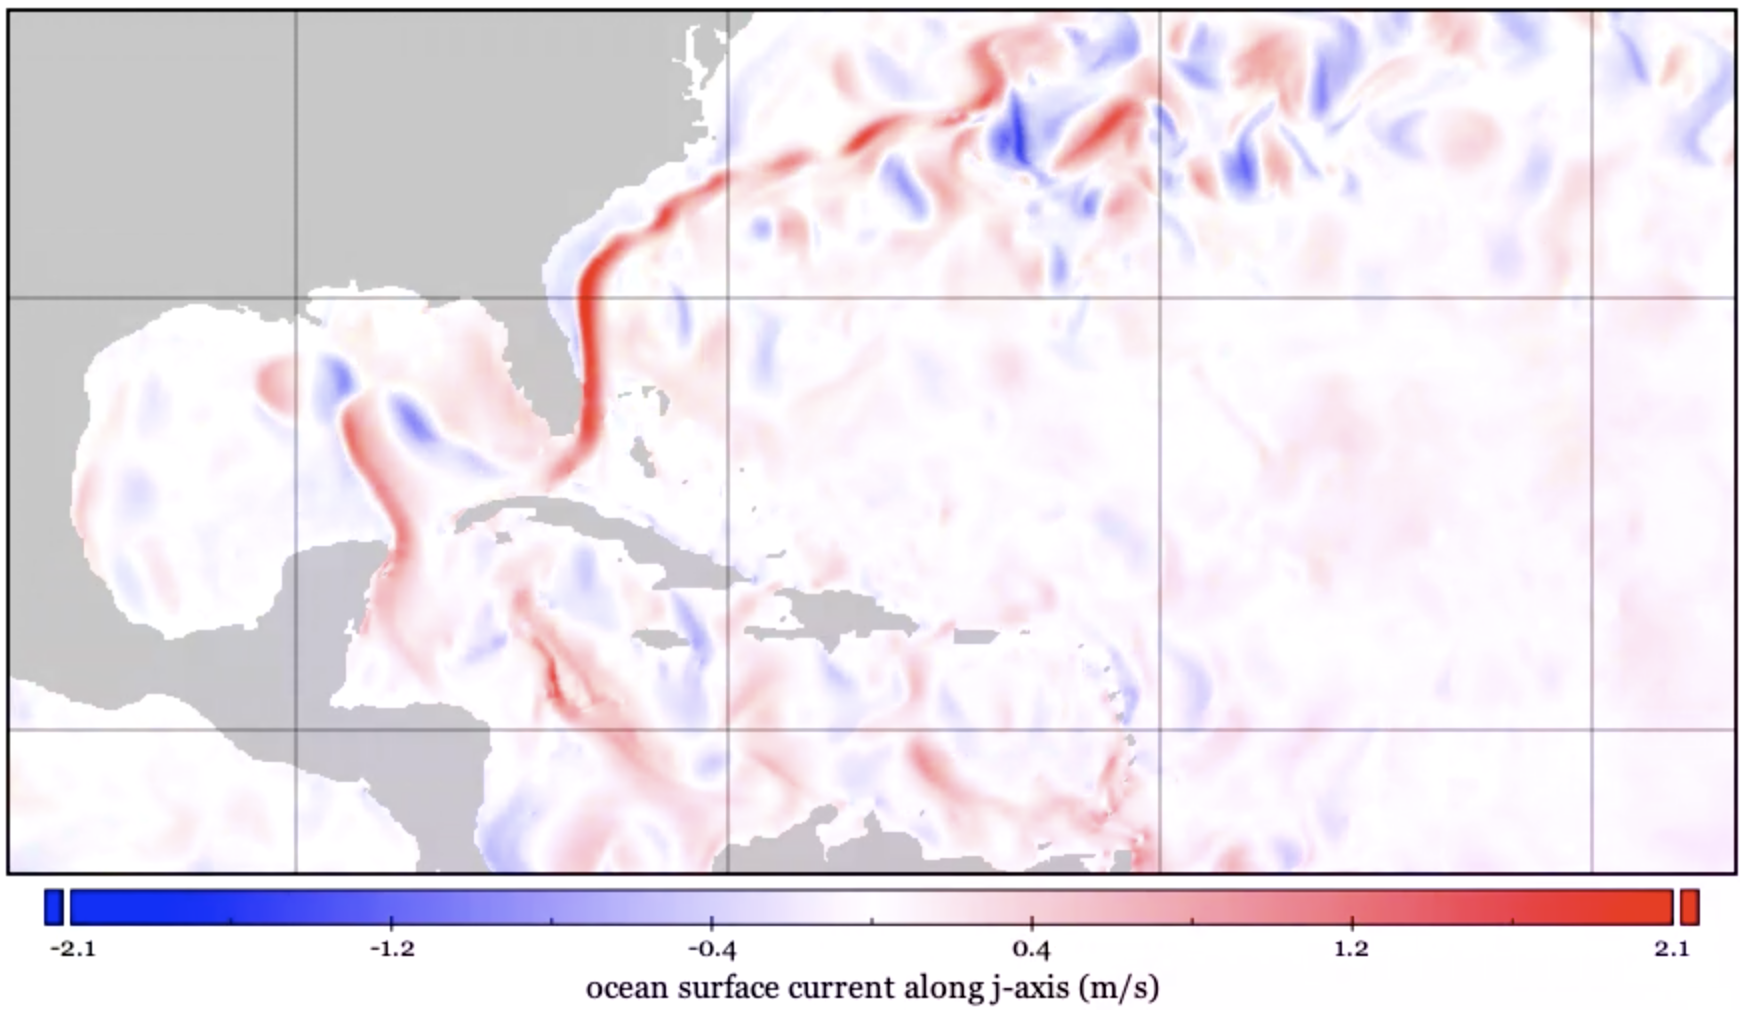
\includegraphics[width=0.93\linewidth]{images/example-images/vos.png}
\caption{Sea surface velocity along Y-axis, (\texttt{vos}, $v$)}
\label{fig:vos}
\end{figure}

\begin{figure}
\vspace{-10pt}
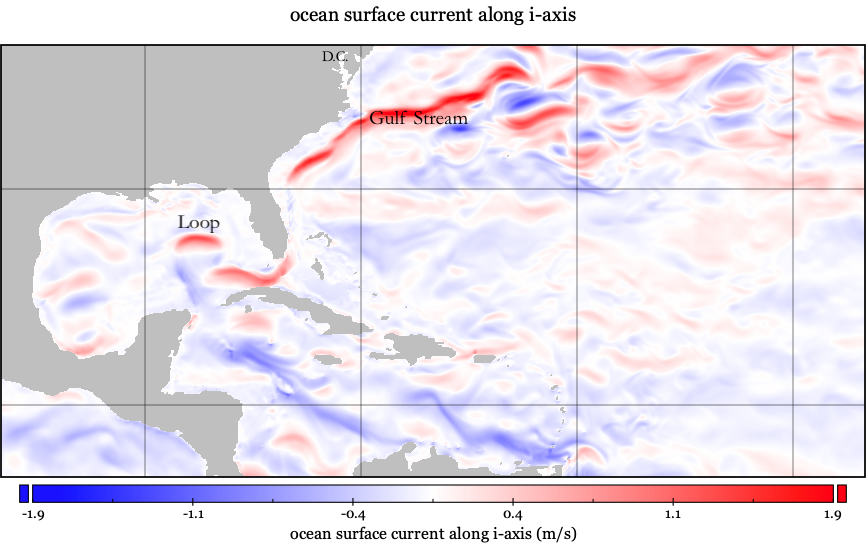
\includegraphics[width=\linewidth]{images/example-images/uos.png}
\caption{Sea surface velocity along X-axis,
         (\texttt{uos}, $u$) from \texttt{tyr}
         on 4th August 2005. }
\label{fig:uos}
\end{figure}



\begin{figure*}
\includegraphics[width=0.48\linewidth]{../surge/plots/low_pass_grid.pdf}
     \includegraphics[width=0.48\linewidth]{../surge/plots/high_pass_grid.pdf}
\caption{Fourier Transform~\cite{cooley1965algorithm} of SSH demeaned by
         coastal point, and low (left) and high (right) pass filtered respectively,
         with a threshold of 2 yr$^{-1}$ (justified by
         Figure~\ref{fig:lpredthresh}). Although not noticeably different in
         the low pass filter (left), Miami and other headlands
         are noticeably less variable in the high pass filter. }
\label{fig:four-trans-panels}
\centering
\includegraphics[width=0.8\linewidth]{../surge/plots/norlean-low-pass.pdf}
\vspace{-10pt}

\caption{New Orleans (NO) closest coastal cell divided
         into high and low frequency components.}
\label{fig:no-hp-lp}


\includegraphics[width=0.8\linewidth]{../surge/plots/mm-low-pass.pdf}
\vspace{-10pt}

\caption{Miami (MM) has more low frequency noise.
         Both this and Figure~\ref{fig:no-hp-lp} above
         show an increase in the low amplitude signal with time,
         which could be explained by the spin
         up of \texttt{tyr} from EN4.}
\label{fig:mm-hp-lp}

\end{figure*}



\begin{figure*}
\centering

\vspace{-35pt}
       \includegraphics[width=0.27\linewidth]{../surge/plots/reg_fft/up_to_100_full_coast.png}
        \includegraphics[width=0.35\linewidth]{../surge/plots/reg_fft/up_to_100_coastal_average.png}
            \caption{\texttt{eUS-tyr} An averaged $r^2$ between \texttt{huber} and \texttt{MLR} trained on 2004 and 2005,
                    and tested on the opposite year (see §~\ref{sec:responsiveness}).}
            \label{fig:lpredthresh}

\begin{minipage}{0.45\textwidth}
\includegraphics[width=1\linewidth]{../surge/plots/lag/fft_pp_zos.png}
            \includegraphics[width=\linewidth]{../surge/plots/lag/zm_fft_pp_zos.png}
            \caption{\texttt{eUS} for \texttt{tyr} demeaned SSH, $\Delta\eta$, fourier transform. Bottom plot is a zoomed in version of the upper.}
            \label{fig:zm_fft_zos}
            \end{minipage}\begin{minipage}{0.45\textwidth}

        \includegraphics[width=1\linewidth]{../surge/plots/lag/fft_pp_tos.png}
            \includegraphics[width=\linewidth]{../surge/plots/lag/zm_fft_pp_tos.png}
            \caption{\texttt{eUS} for \texttt{tyr} demeaned SST, $\Delta T_s$, fourier transform,
                     showing power c.~uniquely located in annual signal.}
            \label{fig:zm_fft_tos}
            \end{minipage}

\end{figure*}


\label{sec:lag}

\begin{figure*}
\includegraphics[width=1\linewidth]{../surge/plots/temp/ssh_sst_grid.pdf}
\caption{There is some interesting structure downstream of Miami, could this be
         movements in the Florida current?
         If so, could it be predictive of the SSH upstream}
         \label{fig:ssh-sst}

\centering
\includegraphics[width=0.45\linewidth]{../surge/plots/lag/correlate_dmdm.pdf}
         \caption{Lag correlation plot}
         \label{fig:lag-plot}
\end{figure*}


To explain this seasonal cycle in SSH, we can see by comparing SST and SSH, as in Figure~\ref{fig:ssh-sst}
for \texttt{eUS} for \texttt{tyr}, that they may be related,
and so we use lag correlation on $\Delta\eta_{\;\mathrm{lp}}(t)$ and SST.
Figure~\ref{fig:lag-plot} (\texttt{eUS}, \texttt{tyr}) tells a simple story of
SSH lagging 30-50 days behind SST, as the mixed layer takes longer
to heat up than the surface.
However Figure~\ref{fig:vc_lag-plot} for \texttt{vc} undermines this as the
lag becomes anti-phase, showing that this is not generally as simple.
Figure~\ref{fig:lpredthresh} justifies removing the low frequency
component of the signal, as it cannot be predicted by sea surface stress.

\FloatBarrier
